\chapter{Superconductivity and quench: an overview}
\label{chp:soupcond-quench}
In this chapter I will explain some of the very basic concepts linked to superconductors and
superconductor quench.
\section{Superconductivity in theory}
\label{sec:soupcond}
Electrical motion in metallic or insulating materials is a very well studied and documented
phenomenon. Electrons passing through any material, endure a varying amount of disturbance in their
motion based on the type of material, this disturbance is known as resistivity $\rho$.
Given a sample of a material of length $l$ and cross-section $A$ we can compute the resistivity as
shown in \ref{eq:resistivity-cable}
\begin{equation}
	\label{eq:resistivity-cable}
	\rho = \frac{RA}{l} = \frac{m}{n\mathcal{e}^2\tau}
\end{equation}
The second part of equation \ref{eq:resistivity-cable} highlights the fact that the resistivity of a
material can be seen as a function of:
\begin{itemize}
	\item The mass of the electron $m$,
	\item The charge density $n$,
	\item The charge of the electron $\mathcal{e}$
	\item The relaxation time of the electron, which is the time interval occurring between two
	      successive collisions between electrons $\tau$.
\end{itemize}

The resistivity of any material at a certain temperature $\rho_T$ can be written as a function of
the sample's resistivity at a certain temperature of reference $\rho_0$ and a regularization term
known as the temperature coefficient of resistivity, which is the ration of resistance change to
temperature change.
\begin{equation}
	\label{eq:resistivity-func-of-temp}
	\rho_T = \rho_0[1 + \alpha(T - T_0)]
\end{equation}

Based on their values of resistivity materials can be divided between metals and insulators. Metals
will have a very low value of resistivity (usually lower than $10^{-5}$) while insulators strongly
oppose to current passing through them.
In \cite{slimani2022superconducting} solid band theory is used in conjunction with equation \ref{eq:resistivity-func-of-temp} behavior of metals and insulators can be explained in terms
of the freedom of movement of electrons in the crystal. An increase in temperature for a metal
translates into an increase in resistivity while insulators experience a decrease in resistivity
and some start behaving like metals \cite{slimani2022superconducting}.

In 1911 \cite{invention-superconductivity} it was discovered that if a sample of mercury was cooled
until it reached the temperature of $4.2K$ the resistance exerted by the sample on a current travelling
through it fell from a definite real value to $0$, as can be
seen in \ref{img:mercury-resistance}, the mercury sample had reached the superconducting state.
\begin{figure}
	\centering
	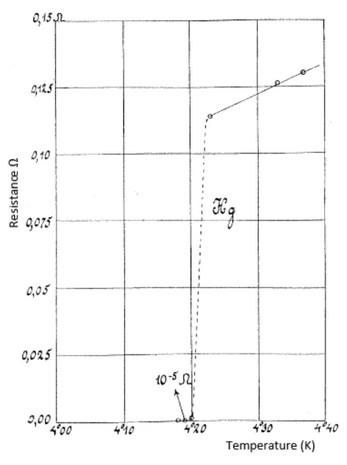
\includegraphics[width=0.5\textwidth]{./img/mercury-resistance.png}
	\caption{The resistance of Mercury in function of the temperature of the sample, taken from
		\cite{tsukerman2020compendium}}
	\label{img:mercury-resistance}
\end{figure}
More studies showed that the material in superconducting state was able to repel materials and, due
to the absence of resistance, allowed the transportation of extremely high currents
\cite{slimani2022superconducting}.

Any material can be kept in the superconducting state as long as:
\begin{itemize}
	\item The temperature of the sample doesn't exceed the critical temperature $\tc$,
	\item The current density passing through the sample doesn't exceed the critical current
	      density $\jc$,
	\item The magnetic field acting on the material doesn't exceed the critical magnetic field $\bc$.
\end{itemize}

When a material reaches the superconducting state it exhibits perfect diamagnetism, which means that
the material is able to perfectly repel magnetic fields, a simple experimental proof of this effect
is given by magnetic levitation. This capacity to repel magnetic fields was first observed by
Meissner and Ochsenfeld in 1933 \cite{meissner1933}. While the repulsion of the magnetic field is
perfect it had already been proven by Geertruida de Haas-Lorentz in 1925 \cite{fokker1925physica} that magnetic fields do, in fact, penetrate the surface of the superconductor and in 1935 the original observation were confirmed by the London's equations \cite{london1935}.

In the following I will be explaining the concepts of Critical temperature, current dencity and
magnetic field.

\subsection{Temperature in superconductors}
\label{sus:temp-soupcond}
The critical temperature of a material is the main aspect to be considered when trying to
characterize its superconductivity properties.

\section{Type I superconductors}
\label{sec:type1}
\section{Type II superconductors}
\label{sec:type2}
